\documentclass[../manuale-utente.tex]{subfiles}

\begin{document}

\subsection{Requisiti}%
\label{sub:requisiti}

\begin{description}
    \item[Sistema operativo:] Android 5.0 o superiore.
    \item[Processore:] ARM32, ARM64, x86, x86\_64.
    \item[Geolocalizzazione:] A-GPS obbligatorio, Glonass e Galileo consigliati.
    \item[Sensori:] Giroscopio, Accelerometro.
\end{description}


\subsection{Manuale d'uso}%
\label{sub:manuale-uso-mobile}

\subsubsection{Pagina di accesso}%
\label{sub:pagina-di-accesso}

\begin{figure}[H]
    \centering
    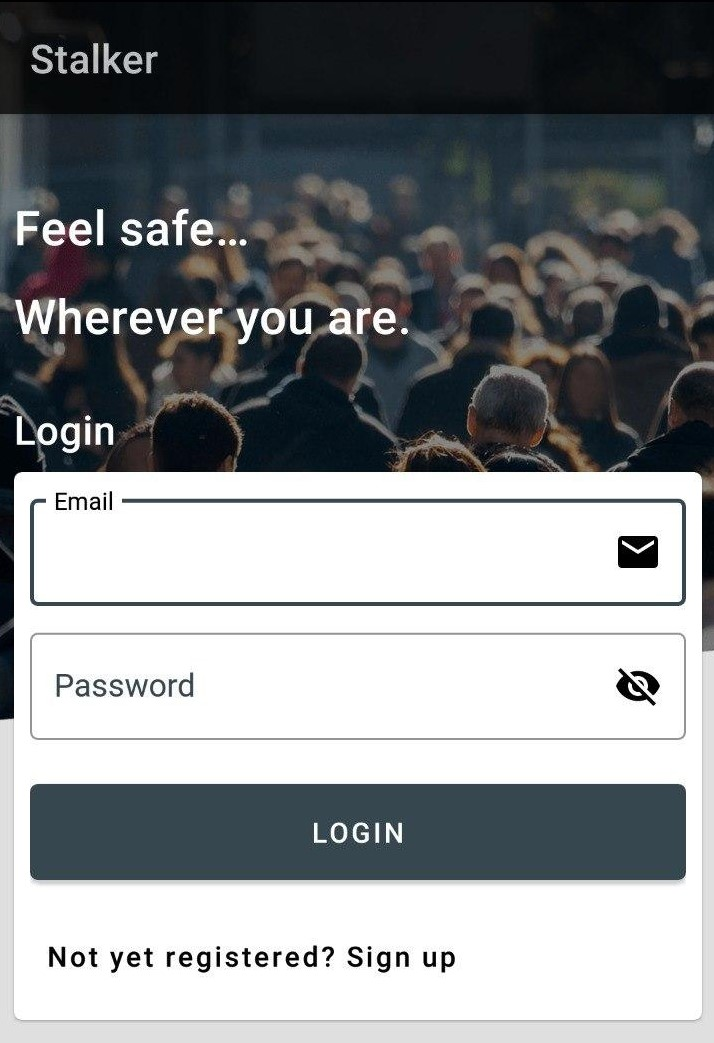
\includegraphics[width=70mm]{img/mobile-app/pagina-di-accesso.jpg}
    \caption{Pagina di accesso}%
    \label{fig:mobile-app-pagina-di-accesso}
\end{figure}

Lorem ipsum

\subsubsection{Pagina di registrazione}%
\label{sub:pagina-di-registrazione}

\begin{figure}[H]
    \centering
    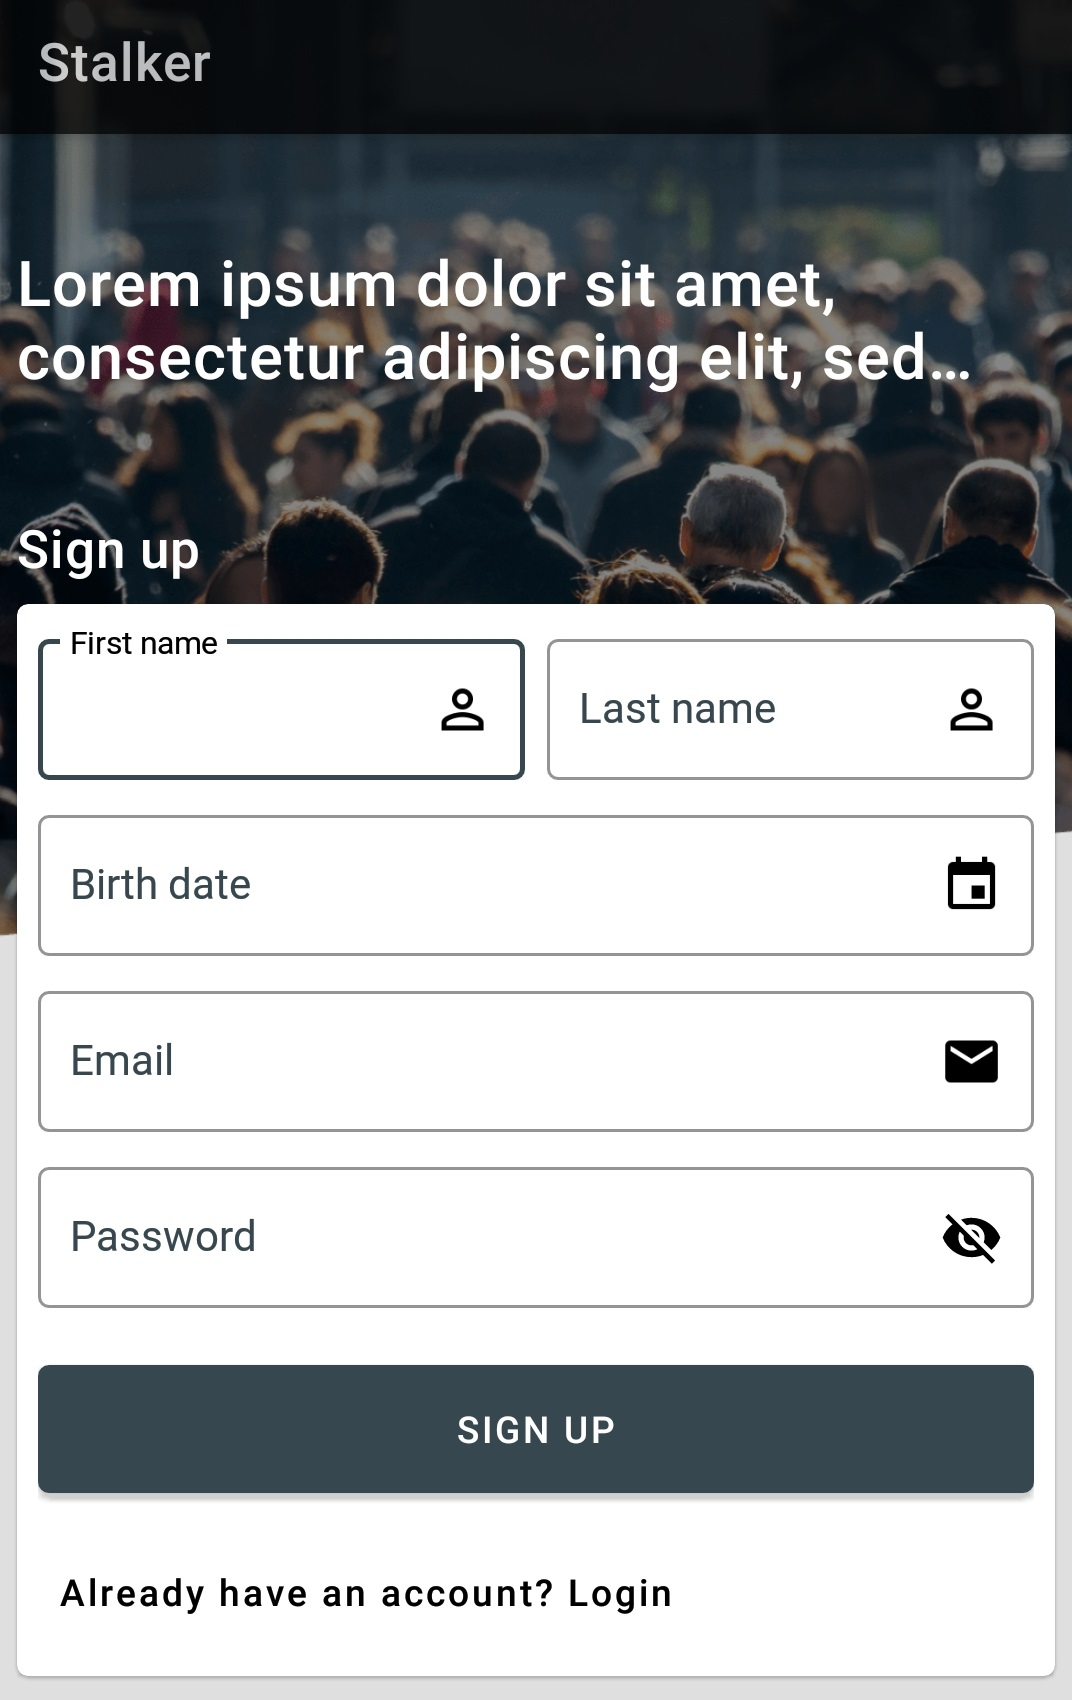
\includegraphics[width=70mm]{img/mobile-app/pagina-di-registrazione.jpg}
    \caption{Pagina di registrazione}%
    \label{fig:mobile-app-pagina-di-registrazione}
\end{figure}

Lorem ipsum

\subsubsection{Pagina iniziale}%
\label{sub:pagina-iniziale}

% \begin{figure}[H]
%     \centering
%     \includegraphics{img/mobile-app/pagina-iniziale.png}
%     \caption{Pagina iniziale}%
%     \label{fig:mobile-app-pagina-iniziale}
% \end{figure}

Lorem ipsum

% add other functionalities 

\end{document}